\documentclass[a4paper,11pt]{article}

\usepackage[utf8]{inputenc}
\usepackage[T1]{fontenc}
\usepackage{graphicx}
\usepackage{amsmath, amssymb}
\usepackage{geometry}
\usepackage{booktabs}
\usepackage{hyperref}
\usepackage{float}
\usepackage{xcolor}
% grffile is often needed for filenames with spaces/dots, though modern engines handle it.
\usepackage[space]{grffile} 
\graphicspath{{img/}} 

\geometry{left=2.5cm, right=2.5cm, top=2.5cm, bottom=2.5cm}

\title{\textbf{R-DARTS: Recursive Differentiable Architecture Search}}
\author{\textbf{Henri d'Andria} \\
\textit{Supervised by Enzo Tartaglione (Telecom Paris)} \\
\textbf{Master's Thesis Project} \\
Institut Polytechnique de Paris}
\date{2022}

\begin{document}

\maketitle

\begin{abstract}
Neural Architecture Search (NAS) has revolutionized deep learning by automating the design of neural networks, traditionally a manual and heuristic-heavy process. While early methods like NASNet achieved state-of-the-art results using Reinforcement Learning, their prohibitive computational cost (thousands of GPU-hours) limited their accessibility. The introduction of DARTS (Differentiable Architecture Search) democratized NAS by relaxing the search space into a continuous domain, allowing gradient-based optimization.

However, most current NAS methods operate on a "flat" search space, assembling networks from a fixed set of primitive operations. This thesis introduces \textbf{R-DARTS} (Recursive DARTS), a hierarchical framework inspired by biological complexity. R-DARTS treats learned architectures not as final outputs, but as new primitive operations for subsequent search iterations. We present a detailed review of the state-of-the-art, reproduce key baselines, and evaluate the viability of this recursive strategy.
\end{abstract}

\section{Introduction}
The field of Deep Learning has long been driven by the manual engineering of architectures. From AlexNet to ResNet and DenseNet, human intuition has defined the topological priors that guide learning. Neural Architecture Search (NAS) proposes to shift this paradigm: instead of designing the network, we design the \textit{process} that builds the network.

Despite their success, NAS algorithms often converge to shallow, repetitive patterns constrained by their primitive operations (typically $3\times3$ or $5\times5$ convolutions). Biological systems, in contrast, exhibit recursion and hierarchy: cells form tissues, tissues form organs, and organs form organisms.

\textbf{Hypothesis:} Can we accelerate the search for optimal macro-structures by recursively assembling locally optimized micro-structures?

This report is structured as follows: Section 2 details the foundational methods (NASNet, DARTS, SETN). Section 3 validates our experimental setup through reproduction. Section 4 analyzes the topological limitations of current methods. Section 5 introduces the R-DARTS methodology, and Section 6 analyzes the results.

\section{State of the Art: A Review}

\subsection{NASNet: The Reinforcement Learning Era}
NASNet \cite{zoph2018learning} is the pioneering work that demonstrated NAS could outperform human-designed networks on ImageNet.

\textbf{Core Innovation:} Separation of Micro and Macro search space.
Instead of searching for the entire network graph (which is too large), NASNet searches for a small building block called a \textbf{"Cell"}. This cell is then stacked $N$ times to create the final network.
\begin{itemize}
    \item \textbf{Normal Cell:} Preserves spatial dimension.
    \item \textbf{Reduction Cell:} Reduces spatial dimension (stride 2).
\end{itemize}

\textbf{Mechanism:} A Recurrent Neural Network (RNN) acts as a \textbf{Controller}. It samples an architecture description as a sequence of discrete parameters (selecting inputs, operations, and combination methods). A child network is built, trained to convergence, and its accuracy is returned as a \textbf{Reward}. The Controller is updated via Reinforcement Learning (PPO) to maximize this reward.

\begin{figure}[H]
    \centering
    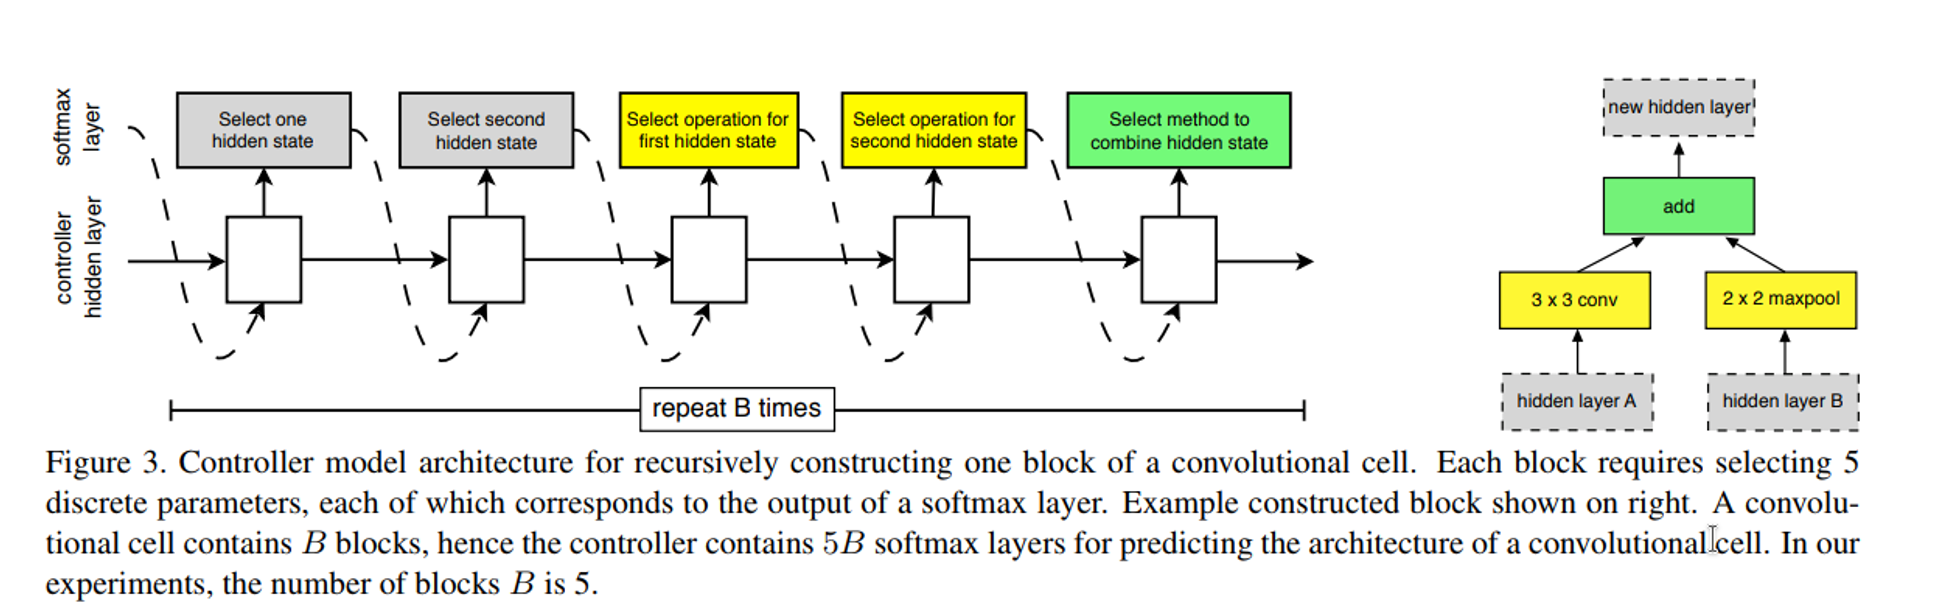
\includegraphics[width=0.9\textwidth]{Nasnet Controller.png}
    \caption{Overview of the NASNet Controller mechanism.}
\end{figure}

\textbf{Limitation:} The primary limitation of this approach lies in its computational inefficiency. The agent requires an extensive exploration of the search space. Since assessing the quality of a single candidate architecture requires training a child network from scratch to convergence, the cumulative computational cost becomes prohibitive ($>500$ GPU-days), making this approach feasible only for massive industrial clusters (e.g., Google).

\subsection{DARTS: Differentiable Architecture Search}
DARTS \cite{liu2018darts} solved the efficiency bottleneck of NASNet by making the search space \textbf{continuous}.

\textbf{Core Innovation:} Continuous Relaxation.
Instead of making a discrete choice (e.g., "Use Conv3x3"), DARTS places \textit{all} possible candidate operations on every edge of the graph. The output of an edge is a weighted sum of all operations:
\begin{equation}
    \bar{o}^{(i,j)}(x) = \sum_{o \in \mathcal{O}} \frac{\exp(\alpha_o^{(i,j)})}{\sum_{o' \in \mathcal{O}} \exp(\alpha_{o'}^{(i,j)})} o(x)
\end{equation}
where $\alpha$ are the architecture parameters.

\vspace{0.5em}
\textbf{Mechanism:} This relaxation makes the objective function differentiable with respect to $\alpha$. DARTS solves a \textbf{bi-level optimization problem}:
\begin{enumerate}
    \item Update network weights $w$ to minimize training loss $\mathcal{L}_{train}$.
    \item Update architecture parameters $\alpha$ to minimize validation loss $\mathcal{L}_{val}$.
\end{enumerate}
At the end of the search, the strongest operations ($\text{argmax } \alpha$) are selected to form the discrete genotype.

\begin{figure}[H]
    \centering
    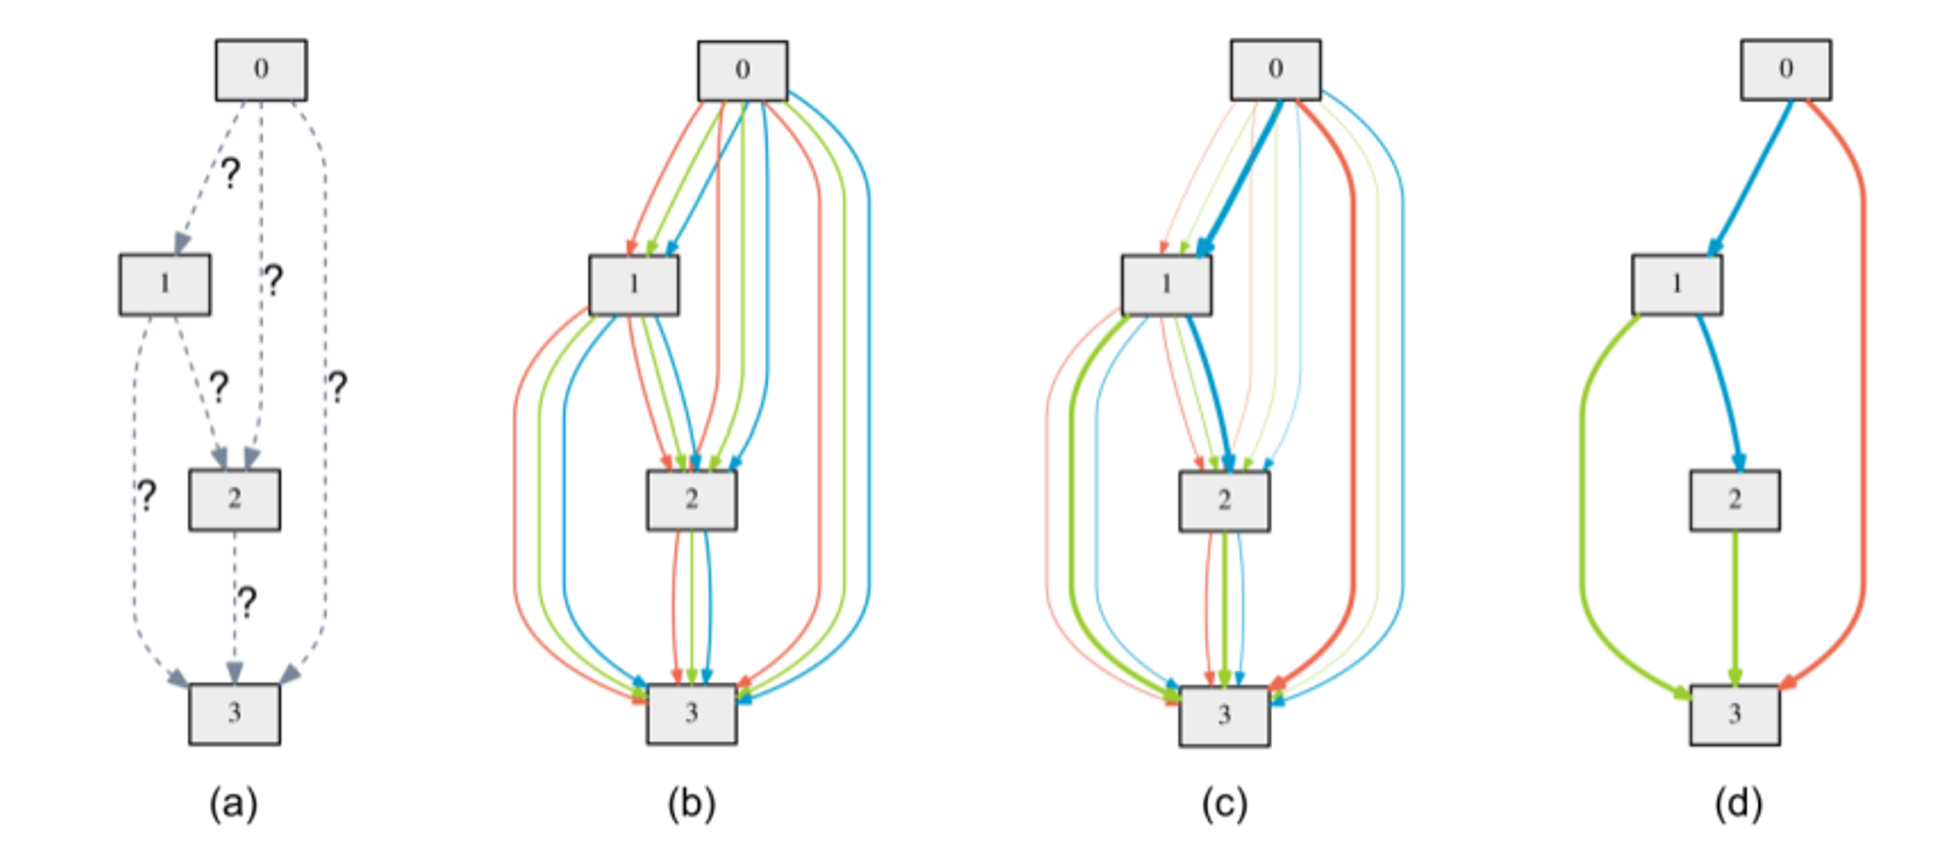
\includegraphics[width=0.8\textwidth]{DARTS - Continuous relaxation.png}
    \caption{The continuous relaxation of the search space. (a) Initially, the operations on the edges are unknown. (b) Continuous relaxation: a mixture of all candidate operations is placed on each edge. (c) Joint optimization: architecture parameters $\alpha$ are trained alongside weights, strengthening some paths (thicker lines). (d) Final discretization: the strongest operation ($\text{argmax } \alpha$) is selected to form the final discrete cell.}
\end{figure}

This fundamental shift from discrete to continuous optimization dramatically reduced the computational burden, lowering the search cost from 500 to just \textbf{4 GPU-days}.

\subsection{SETN: One-Shot Approach}
SETN \cite{dong2019one} addresses the bias introduced by the weight-sharing in DARTS and the cost of NASNet.

\textbf{Core Innovation:} Self-Evaluated Template Network.
SETN proposes a "One-Shot" approach where a single super-network (Template) is trained. Instead of bi-level optimization (DARTS) or training thousands of children (NASNet), it trains an \textbf{Evaluator} alongside the network.
\begin{itemize}
    \item The Evaluator learns to predict the accuracy of a random architecture sampled from the Template.
    \item This avoids the expensive retraining of candidates during the search.
\end{itemize}

\textbf{Assessment:} SETN offers a competitive trade-off, achieving state-of-the-art accuracy with a search cost lower than DARTS (1.8 GPU-days). However, for this thesis, we selected DARTS as our foundation. Its gradient-based nature allows for a more natural integration of recursive structures (backpropagation through nested cells) compared to the stochastic sampling and estimator training required by SETN.

\section{Experimental Reproduction}
To establish a reliable baseline for our Master's project, we first reproduced the results of the reference papers on the CIFAR-10 dataset.

\begin{table}[H]
\centering
\begin{tabular}{lcccc}
\toprule
\textbf{Method} & \textbf{Search Cost} & \textbf{Params} & \textbf{Error (CIFAR-10)} & \textbf{Status} \\
& (GPU-days) & (M) & (\%) & \\
\midrule
NASNet \cite{zoph2018learning} & 500 & 3.3M & 2.65 & Reference \\
DARTS \cite{liu2018darts} & 3.0 & 3.3M & 3.00 & Reference \\
\textbf{DARTS (Ours)} & \textbf{2.06} & \textbf{3.34M} & \textbf{2.57} & \textbf{Reproduced} \\
SETN \cite{dong2019one} & 1.8 & 4.6M & 2.69 & Reference \\
SETN (Ours) & 1.45 & 4.62M & 3.00 & Reproduced \\
\bottomrule
\end{tabular}
\caption{Baseline reproduction results. Our reproduction of DARTS achieved even better efficiency and accuracy than reported, validating our codebase as a solid foundation for R-DARTS.}
\label{tab:repro}
\end{table}

\section{Problem Statement: Limitations of Flat Topology}
Despite their impressive results, current NAS methods (including DARTS) suffer from a fundamental topological limitation: \textbf{Flatness}.

The search process assumes that the final network is a linear stack of identical cells. While the \emph{micro-structure} (the cell itself) is optimized, the \emph{macro-structure} is rigid. This "brute-force encapsulation" prevents the emergence of sophisticated patterns found in state-of-the-art manual designs:

\begin{itemize}
    \item \textbf{Lack of Long-Range Connections:} Architectures like ResNet or DenseNet rely on skip-connections that span across many layers. In DARTS, a skip-connection is strictly local (within a cell). The algorithm cannot decide to connect Layer 5 directly to Layer 10 unless the human engineer hard-codes it.
    \item \textbf{Rigid Hierarchy:} Models like U-Net rely on multi-scale interactions (contracting and expansive paths). DARTS cannot "discover" a U-Net shape; it can only discover the building block of a U-Net, but the U-shape itself must be predefined.
\end{itemize}

This limitation motivates the need for \textbf{R-DARTS}. By allowing the algorithm to encapsulate a complex subgraph into a single operation, we enable the discovery of hierarchical dependencies and macro-structures that are currently out of reach.

\section{R-DARTS: The Proposal}

\subsection{Recursive Methodology}
The R-DARTS algorithm iterates on the search process:
\begin{enumerate}
    \item \textbf{Iteration 0:} Run standard DARTS with atomic primitives $\mathcal{O}_0 = \{\text{conv3x3}, \text{maxpool}, \dots\}$.
    \item \textbf{Extraction:} Select the top-$k$ best cell structures (Genotypes $G_0^1, \dots, G_0^k$) based on learned $\alpha$, ensuring diversity in the new primitive set.
    \item \textbf{Encapsulation:} Wrap each selected genotype into a new differentiable operation, `CellOp`. These operations behave like standard layers but internally contain the complex graphs of their respective genotypes.
    \item \textbf{Iteration 1:} Define a new search space $\mathcal{O}_1 = \{\text{none}, G_0^1, \dots, G_0^k\}$. (\textit{Note:} \texttt{none} is the zero/skip operation kept as in DARTS to allow pruning/sparsity.) We set $k = |\mathcal{O}_0|$ (typically 8) to keep the search space size and optimization dynamics comparable.
    \item \textbf{Search:} Run DARTS again. The algorithm can now choose to insert entire pre-optimized cells as atomic operations, combining different specialized structures.
\end{enumerate}

\paragraph{Transition Strategy: Diversity vs. Optimality.}
A crucial aspect of R-DARTS is how we transition between levels. We employ two distinct strategies for extracting genotypes from the learned architecture weights $\alpha$:
\begin{itemize}
    \item \textbf{Deterministic Selection (Evaluation):} To obtain the single best architecture for final training, we select the operation with the highest weight ($\text{argmax } \alpha$) on each edge. This yields the most optimized structure found during the search.
    \item \textbf{Stochastic Sampling (Recursion):} For the recursive step, relying solely on the best architecture would impoverish the search space. Instead, we sample $k$ distinct genotypes from the softmax distribution of the architecture weights. This probabilistic approach ensures structural diversity in the new primitive set $\mathcal{O}_{level+1}$, preventing the algorithm from converging prematurely to a single pattern.
\end{itemize}

\subsection{Technical Challenge: The Dimensional Mismatch}
A major challenge in R-DARTS arises from the rigid dimensional constraints of the original DARTS framework.

\paragraph{Standard DARTS constraints.}
In the original implementation, the search space consists of two distinct cell types:
\begin{itemize}
    \item \textbf{Normal Cells:} Maintain the spatial resolution ($H \times W$) and number of channels ($C$).
    \item \textbf{Reduction Cells:} Reduce the spatial resolution by half ($H/2 \times W/2$) and double the channels ($2C$).
\end{itemize}
Crucially, a cell at layer $k$ receives inputs from layers $k-1$ and $k-2$. Because Reduction cells alter dimensions, these two inputs often have different shapes (e.g., if layer $k-1$ was a reduction cell, input $k-2$ is twice as large as input $k-1$).

\paragraph{The Recursive Conflict.}
In R-DARTS, we encapsulate an entire cell structure into a single primitive operation (e.g., a "Normal Cell" from Level 0 becomes a "LayerOp" in Level 1). This creates a conflict:
\begin{enumerate}
    \item \textbf{Stride Incompatibility:} If a Level 0 "Normal Cell" (designed for stride 1) is selected as an operation inside a Level 1 "Reduction Cell" (which demands stride 2), the internal structure must be forced to perform a downsampling it wasn't originally designed for.
    \item \textbf{Channel Mismatch:} Recursive operations may be inserted at any depth. An operation learned with 16 channels at Level 0 might be instantiated with 64 channels at Level 1, requiring robust internal channel scaling.
\end{enumerate}

\paragraph{Solution: Adaptive Preprocessing.}
To resolve this, we generalized the preprocessing logic of DARTS. Before entering the recursive core, inputs are passed through adaptive layers that normalize their dimensions:
\begin{itemize}
    \item \textbf{ReLU-Conv-BN:} Projects channel dimensions (e.g., $4C \to C$) without changing spatial resolution.
    \item \textbf{FactorizedReduce:} Handles spatial downsampling (stride 2) while preserving information. Unlike a standard strided convolution, it uses two shifted $1\times1$ convolutions to cover the entire spatial field before concatenation.
\end{itemize}
By systematically wrapping recursive primitives with these adapters, we ensure that any cell topology from Level $L-1$ can be plugged into any slot (Normal or Reduction) at Level $L$.

\begin{figure}[H]
    \centering
    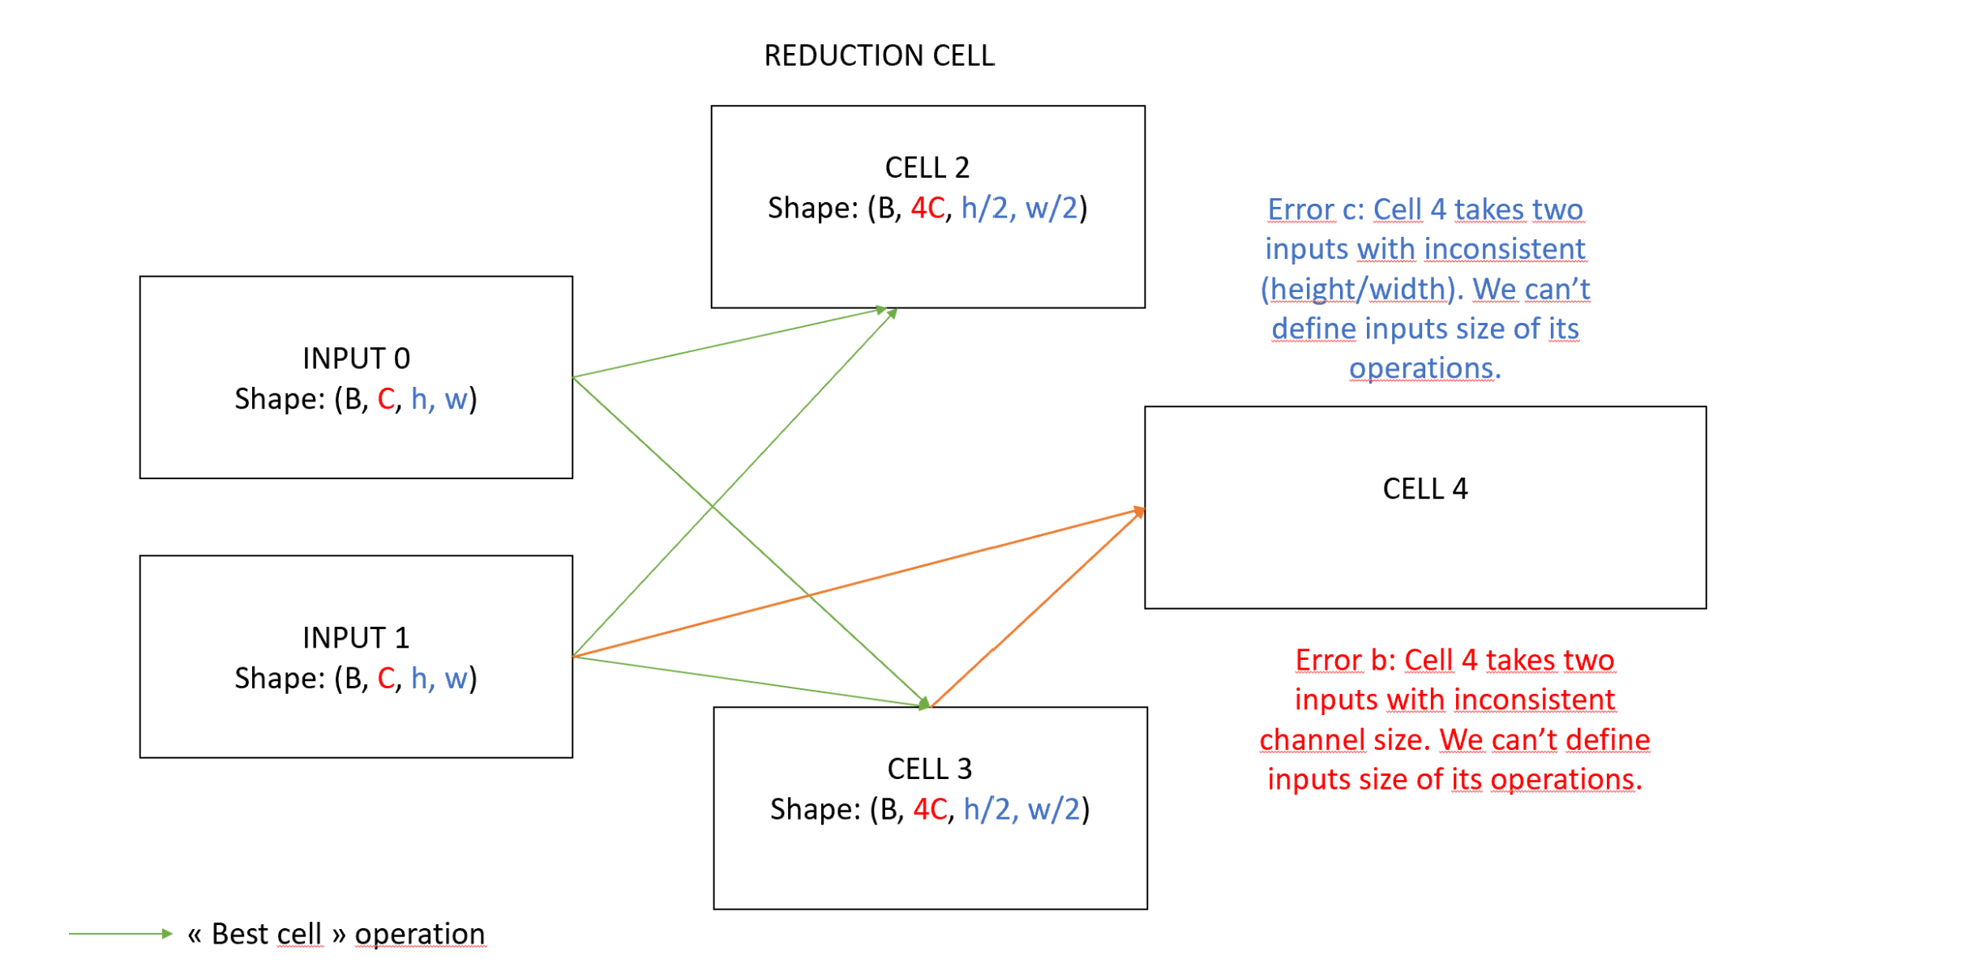
\includegraphics[width=0.9\textwidth]{RDARTS - Dimension mismatch.png}
    \caption{Visualizing the dimensional mismatch challenge when nesting cells. The red and blue errors highlight where the input tensors (from previous layers) clash with the internal cell operations due to inconsistent resolutions or channel depths.}
\end{figure}

\section{Results: R1-DARTS}
We trained a first-level recursive architecture (R1-DARTS) on CIFAR-10.

\begin{table}[H]
\centering
\begin{tabular}{lccc}
\toprule
\textbf{Model} & \textbf{GPU-days} & \textbf{Params} & \textbf{Error (\%)} \\
\midrule
DARTS (Base) & 2.06 & 3.34M & 2.57 \\
\textbf{R1-DARTS} & \textbf{2.6} & \textbf{3.1M} & \textbf{5.5} \\
\bottomrule
\end{tabular}
\caption{Preliminary results for Recursive DARTS.}
\end{table}

\subsection{Analysis}
The slight increase in search cost (2.6 vs 2.06 days) reflects a conscious design choice: \textbf{we enforced a strict computational budget}. To keep R-DARTS comparable to the baseline, we reduced the number of search epochs for the Level 0 (primitive generation) phase.

\begin{itemize}
    \item \textbf{Impact of Limited Budget:} Reducing the search time for Level 0 likely produced sub-optimal primitives. The algorithm had to build a complex recursive structure on top of "weak" foundations, contributing to the higher error rate (5.5\%).
    \item \textbf{Optimization Instability:} The bi-level optimization problem in DARTS is known to be unstable. Recursively nesting cells deepens the computation graph, exacerbating this instability and making the joint optimization of weights and architecture parameters significantly harder to converge.
    \item \textbf{Expressivity vs. Trainability:} The resulting topology was "richer" but harder to train from scratch.
\end{itemize}

\clearpage
\section{Conclusion \& Future Work}
This thesis project successfully implemented a functional Recursive NAS pipeline. We demonstrated that cells can be technically treated as primitives. The performance gap suggests that while the \textit{topology} is valid, the \textit{optimization strategy} needs adaptation for recursive structures.

\textbf{Future directions:}
\begin{itemize}
    \item \textbf{Unary Restrictions:} Limit recursive cells to unary operations. Standard DARTS cells are designed with two inputs ($k-1, k-2$), which forces us to duplicate the single input when wrapping them as atomic primitives. Constraining the inner search space to unary topologies would align strictly with the definition of a standard layer operation.
    \item \textbf{Differential Learning Rates:} Instead of training all levels at the same rate, applying a lower learning rate to the inner weights of the recursive primitives could stabilize the optimization of the hierarchical structure.
    \item \textbf{Enriched Search Spaces:} Enrich the primitive set with heavier, state-of-the-art blocks such as Self-Attention modules or Transformer layers, allowing the search to discover more diverse and powerful architectures beyond standard CNN patterns.
\end{itemize}

\begin{thebibliography}{9}

\bibitem{liu2018darts}
Liu, H., Simonyan, K., \& Yang, Y. (2018).
\textit{DARTS: Differentiable Architecture Search}.
arXiv preprint arXiv:1806.09055.

\bibitem{zoph2018learning}
Zoph, B., Vasudevan, V., Shlens, J., \& Le, Q. V. (2018).
\textit{Learning Transferable Architectures for Scalable Image Recognition}.
Proceedings of the IEEE Conference on Computer Vision and Pattern Recognition, 8697--8710.

\bibitem{dong2019one}
Dong, X., \& Yang, Y. (2019).
\textit{One-Shot Neural Architecture Search via Self-Evaluated Template Network}.
Proceedings of the IEEE/CVF International Conference on Computer Vision, 3681--3690.

\end{thebibliography}

\end{document}
